\documentclass[varwidth=true, border=2pt]{standalone}

\usepackage{pgfplots}
\usepackage{tikz}

\usetikzlibrary{calc,patterns,angles,quotes}

\begin{document}
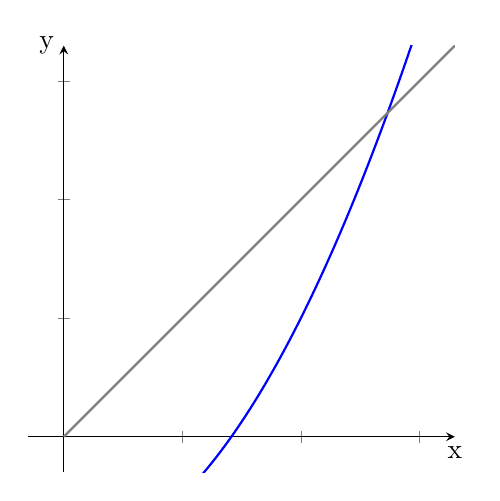
\begin{tikzpicture}
    \begin{axis}[
        legend pos=south east,
        axis x line=middle,
        axis y line=middle,
	every axis x label/.style={at={(current axis.right of origin)},anchor=north},
	every axis y label/.style={at={(current axis.above origin)},anchor=east},
	xticklabels=\empty,
	yticklabels=\empty
        grid = none ,
        width=7cm,
        height=7cm,
        grid style={dashed, gray!1},
        xmin=0,     % start the diagram at this x-coordinate
        xmax= 3,    % end   the diagram at this x-coordinate
        ymin=0,     % start the diagram at this y-coordinate
        ymax= 3,   % end   the diagram at this y-coordinate
        xlabel=x,
        ylabel=y,
        enlargelimits=true,
        tension=0.08]

        \addplot[domain=-0:8,blue, thick,samples=250] {0.5*x^2-1}; % Parabola
         \addplot[domain=-0:8, gray, thick,samples=250] {x};


%	\addplot[dashed,red,mark=none] coordinates{(1,0)(1,1.316)} node[below, pos=0] {$x_0$}; %x0
%	\addplot[dashed,red,mark=none] coordinates{(1,1.316)(1.316,1.316)} node[below, pos=0] {};
%	\addplot[dashed,red,mark=none] coordinates{(1.316,1.316)(1.316,1.592)} node[below, pos=0] {};
%	\addplot[dashed,red,mark=none] coordinates{(1.316,1.592)(1.592,1.592)} node[below, pos=0] {};
%	\addplot[dashed,red,mark=none] coordinates{(1.592,1.592)(1.592,1.819)} node[below, pos=0] {};
%	\addplot[dashed,red,mark=none] coordinates{(1.592,1.819)(1.819,1.819)} node[below, pos=0] {};
%	\addplot[dashed,red,mark=none] coordinates{(1.819,1.819)(1.819,1.994)} node[below, pos=0] {};
%	\addplot[dashed,red,mark=none] coordinates{(1.994,1.994)(1.994,2.12)} node[below, pos=0] {};
%	\addplot[dashed,red,mark=none] coordinates{(1.994,2.12)(2.12,2.12)} node[below, pos=0] {};
%	\addplot[dashed,red,mark=none] coordinates{(2.12,2.12)(2.12,2.21)} node[below, pos=0] {};
%	\addplot[dashed,red,mark=none] coordinates{(2.12,2.21)(2.21,2.21)} node[below, pos=0] {};
%	\addplot[dashed,red,mark=none] coordinates{(2.21,2.21)(2.21,2.268)} node[below, pos=0] {};
%	\addplot[dashed,red,mark=none] coordinates{(2.21,2.268)(2.268,2.268)} node[below, pos=0] {};
    \end{axis}
\end{tikzpicture}
\end{document}